\secput{results}{Implementation and Experimentation}
We implemented each of the simple solutions described in 
\secref{simple}, and compared their performance to range coalescing on a variety of data sets. 

Each solution was implemented in C++, and compiled and tested on an Intel i7 processor with 3MB of L3 cache. We implemented the full merge range coalescing solution, instead of the randomized solution. Before each test, $k$ lists each of length $n$ were generated using a uniform distribution from 0 to 1 million. These lists were passed in as input to each of the solutions.  The initialization times and average query times of each solution were recorded. 

Range coalescing performed significantly better in practice than other 
linear-storage solutions. It performed better on both small and large datasets. Average query times are shown in \figref{results-k} and \figref{results-n}.
As the datasets got larger, the effects of range coalescing became more evident. 
For $n=50$ and $k=1000$, range coalescing did 5 times better than a simple binary search,
whereas for $n=5000$ and $k=1000$, range coalescing performed 18 times better.

However, range coalescing requires much more time for initialization. 
It takes about 20 times longer than initialize than the vEB search, and 3 times longer
than fractional cascading. We believe these results could be improved upon - we did not implement the linear time initialization method described here, but we leave that as future work.

The average query time for the quadratic storage solution was better than all 
linear storage solutions. However, it required $O(nk^2)$ time to initialize. For $k=1000,n=100$, this took 42 times longer than range coalescing to initialize.


\begin{figure}
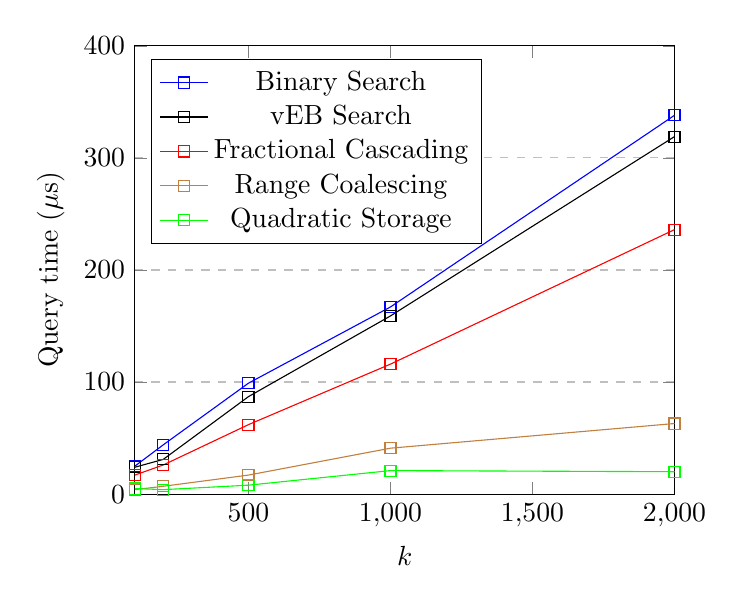
\begin{tikzpicture}
\begin{axis}[
    %title={},
    xlabel={$k$},
    ylabel={Query time ($\mu$s)},
    xmin=100, xmax=2000,
    ymin=0, ymax=400,
    legend pos=north west,
    ymajorgrids=true,
    grid style=dashed,
]
 
  \addplot[color=blue,mark=square] coordinates {(100,25)(200,44)(500,99)(1000,167)(2000,338)};
    \addlegendentry{Binary Search}
 
  \addplot[color=black,mark=square] coordinates {(100, 24) (200, 31) (500,87)(1000,159)(2000,319)};
    \addlegendentry{vEB Search};

  \addplot[color=red,mark=square] coordinates {(100, 17) (200, 26)(500,62)(1000,116)(2000,236)};
    \addlegendentry{Fractional Cascading}

  \addplot[color=brown,mark=square] coordinates {(100, 4) (200, 7)(500,17)(1000,41)(2000,63)};
    \addlegendentry{Range Coalescing};
  \addplot[color=green,mark=square] coordinates {(100, 5) (200, 4)(500,8)(1000,21)(2000,20)};
    \addlegendentry{Quadratic Storage};
\end{axis}
\end{tikzpicture}
\caption{Query times vs $k$ (for fixed $n$=1000).}
\label{fig:results-k} 
\end{figure}

\begin{figure}
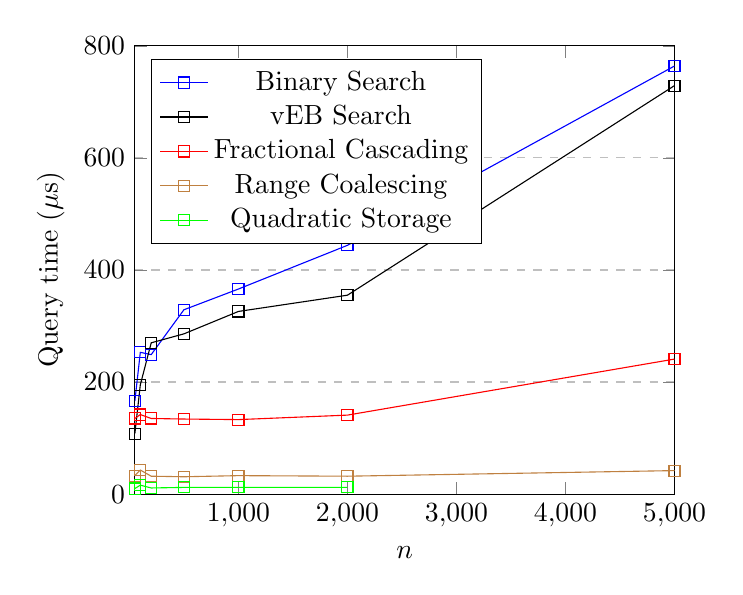
\begin{tikzpicture}
\begin{axis}[
    %title={},
    xlabel={$n$},
    ylabel={Query time ($\mu$s)},
    xmin=50, xmax=5000,
    ymin=0, ymax=800,
    legend pos=north west,
    ymajorgrids=true,
    grid style=dashed,
]
 
  \addplot[color=blue,mark=square] coordinates {(50,166)(100,253)(200,249)(500,329)(1000,366)(2000,444)(5000,764)};
    \addlegendentry{Binary Search}
 
  \addplot[color=black,mark=square] coordinates {(50,108)(100,195)(200,270)(500,286)(1000,326)(2000,355)(5000,729)};
    \addlegendentry{vEB Search};

  \addplot[color=red,mark=square] coordinates {(50,135)(100,142)(200,135)(500,134)(1000,133)(2000,141)(5000,241)};
    \addlegendentry{Fractional Cascading}

  \addplot[color=brown,mark=square] coordinates {(50,33)(100,43)(200,32)(500,31)(1000,33)(2000,32)(5000,42)};
    \addlegendentry{Range Coalescing};
  \addplot[color=green,mark=square] coordinates {(50,10)(100,16)(200,11)(500,12)(1000,12)(2000,12)};
    \addlegendentry{Quadratic Storage};
\end{axis}
\end{tikzpicture}
\caption{Query times vs $n$ (for fixed $k$=1000).}
\label{fig:results-n} 
\end{figure}

